\documentclass{base}
% Dateikodierung ist utf8
\usepackage[utf8]{inputenc}
\usepackage{url}
\usepackage[export]{adjustbox}
\usepackage{amsmath}
\usepackage{listings}
\usepackage{tikz}
\usepackage{tabularx}
\usepackage{color,colortbl}
\usepackage{ulem}
\usepackage{pdfpages}
\usepackage{ wasysym }
\usepackage{ booktabs }
\usepackage{lscape}
\usepackage{multicol}

\begin{document}

\Abgabeblatt{Assignment 3b}{30.4.2018 / 07.05.2018}{????}{????}{Yannis Rohloff (yannis@uni-bremen.de)}{Meng Liu(lium@uni-bremen.de)}{Peter Tschubij (tschupet@uni-bremen.de)}

\lstset{
    language=Python,
    basicstyle=\ttfamily\small,
    aboveskip={1.0\baselineskip},
    belowskip={1.0\baselineskip},
    columns=fixed,
    extendedchars=true,
    breaklines=true,
    tabsize=4,
    prebreak=\raisebox{0ex}[0ex][0ex]{\ensuremath{\hookleftarrow}},
    frame=lines,
    showtabs=false,
    showspaces=false,
    showstringspaces=false,
    keywordstyle=\color[rgb]{0.627,0.126,0.941},
    commentstyle=\color[rgb]{0.133,0.545,0.133},
    stringstyle=\color[rgb]{01,0,0},
    numbers=left,
    numberstyle=\small,
    stepnumber=1,
    numbersep=10pt,
    captionpos=t,
    escapeinside={\%*}{*)}
}


\section*{Exercise 1: Cutting Fabric - Variable Definition}

In a shorter manner than on the first part of this assignment we define our variables and constraints again. Also we note the things we changed.

Let's clarify a few terms. The \textit{workspace} is rectangular arrangement of \textit{fields}. Each \textit{fields} should be filled by one \textit{tile}, where each \textit{tile} is a part of a shape.

A field is identified by it's coordinates $c = (x,y)$.
Every tile of a shape is represented by a tuple $t = (s, n)$. where $s$ is the shape id it belongs to and $n$ is the tile number within this shape. We removed the third variable that stated the rotation and encode the rotation into the $s$ instead since we will copy every shape from the input four times. We also remove shapes that are equal so we can reduce the variable size a little bit (See Block 0 in the example output below).

Now we can define a Variable stating if a field is occupied by a tile:
$$X_{c,t} = X_{(x,y),(s,n)}$$

Furthermode we will use ladder variables but will not formalize them here since they are defined in the lecture notes.

In the first part of this exercise we assumed that we need to duplicate the workspace. We noticed that this is not the case and it is suficcient to use the modulo operator to make the workspace repeat directly (See Constraint 4).

With $w=2$ and $h=3$ the new extended workspace would be:
\begin{center}
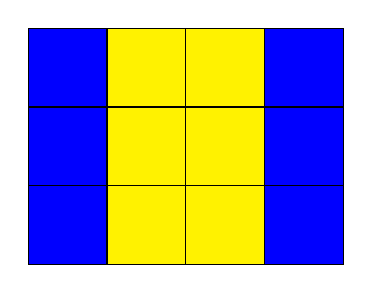
\begin{tikzpicture}[scale=1]
    \draw [fill=blue] (0,3) rectangle (1,4);:
    \draw [fill=yellow] (1,3) rectangle (2,4);
    \draw [fill=yellow] (2,3) rectangle (3,4);
    \draw [fill=blue] (3,3) rectangle (4,4);

    \draw [fill=blue] (0,4) rectangle (1,5);
    \draw [fill=yellow] (1,4) rectangle (2,5);
    \draw [fill=yellow] (2,4) rectangle (3,5);
    \draw [fill=blue] (3,4) rectangle (4,5);

    \draw [fill=blue] (0,5) rectangle (1,6);
    \draw [fill=yellow] (1,5) rectangle (2,6);
    \draw [fill=yellow] (2,5) rectangle (3,6);
    \draw [fill=blue] (3,5) rectangle (4,6);
\end{tikzpicture}
\end{center}

Removing the duplicated workspace results in one of our old constraints to be obsolete. Thus we removed it.

The Constraints mostly stayed the same as before. Except that we used the ladder encoding this time.
We remove the verbose explanation since the constraints are explained in more detail on the first part of this excersie.


\subsection*{Constraint 1: Every field in O has no tile.}
$$\bigwedge_{\substack{c \in O}} \bigwedge_{\substack{t \in T}} \neg X_{c,t}$$

\subsection*{Constaint 2: Excatly one tile per field (With Ladder Encoding)}
We replaced the old constraints 2 and 3 by using the ladder encoding from the course to count the filled fields.

With the ladder encoding we define a helper variable $Y_{c,t}$ for each variable $X_{c,t}$.
Let $(s_0,\dots,s_m)$ be all the shapes and $tiles(s_i)$ the amount of tiles in the shape $s_i$.

$$ \bigwedge_{\substack{c \in F}} \bigwedge_{\substack{m \in \{0,\dots,m\}}}\ \  (X_{c,(m, 0)} \lor -Y_{c,(m, 0)}) \land (-X_{c,(m, 0)} \lor Y_{c,(m, 0)}) $$
\begin{align}
    \bigwedge_{\substack{c \in F}} \bigwedge_{\substack{m \in \{0,\dots,m\}}}\ \ \bigwedge_{\substack{i \in \{0,\dots,tiles(s_m)-2\}}}\ \  &(Y_{c,(m, i+1)} \lor -X_{c,(m, i+1)}) \\
    & \land (Y_{c,(m, i+1)} \lor -Y_{c,(m, i)}) \\
    & \land (-Y_{c,(m, i+1)} \lor X_{c,(m, i+1)} \lor Y_{c,(m, i)}) \\
    & \land (-Y_{c,(m, i)} \lor -X_{c,(m, i+1)})
\end{align}

And finally 
$$\bigwedge_{\substack{c \in F}}\bigwedge_{\substack{m \in \{0,\dots,m\}}}\ \  Y_{c,(m, tiles(s_m)-1)}$$


\subsection*{Constraint 3: If a tile is connected on a field, the neighbors of the field are filled with the neighbors of the tile in the shape.}

$$\bigwedge_{\substack{c \in F}} \bigwedge_{\substack{t \in T}} \neg X_{c,t}$$

Horizontal:
$$\bigwedge_{\substack{(x,y) \in F\cup O}}\ \  \bigwedge_{\substack{(t1,t2) \in H}} \neg X_{(x,y),t1} \lor X_{(x+1,y),t2} $$
Horizontal back implication:
$$\bigwedge_{\substack{(x,y) \in F\cup O}}\ \  \bigwedge_{\substack{(t1,t2) \in H}} X_{(x,y),t1} \lor \neg X_{(x+1,y),t2} $$

Vertical:
$$\bigwedge_{\substack{(x,y) \in F\cup O}}\ \  \bigwedge_{\substack{(t1,t2) \in V}} \neg  X_{(x,y),t1} \lor X_{(x,(y+1)\%h),t2} $$
Vertical back implication:
$$\bigwedge_{\substack{(x,y) \in F\cup O}}\ \  \bigwedge_{\substack{(t1,t2) \in V}} X_{(x,y),t1} \lor \neg X_{(x,(y+1)\%h),t2} $$

We don't have two workspaces anymore. Instead we besically let the one workspace wrap around by using modulo on the y-axis.

\subsection*{Order of Variables}
The order of the variables is important to how fast the sat solver is able to solve the formula.
We considered three orders of variables. \\
Let $o_1,\dots o_{|O|\cdot |T|}$ be the border variables.\\
Let $f_1,\dots f_{|F|\cdot |T|}$ be the inner field variables.\\
Let $y_1,\dots f_{|Y|\cdot |T|}$ be the ladder encoding variables.\\
$ord_1 = (o_1,\dots, f_1,\dots, y_1,\dots)$ \\
$ord_2 = (o_1,\dots, y_1,\dots, f_1,\dots)$ \\
$ord_3 = (o_1,\dots, f_1,y_1,f_2,y_2,\dots)$ \\

To benchmark these we tried all orders on a slightly smaller Problem instance of the 400\dots cnf.
We noticed that $ord_2$ is the by far the fastest.


\subsection*{Benchmark}

We tested our algorithm with the given example problem instances.
Furthermore we compared the execution times even though they heavily depend on the cpu.

To benchmark our algorithm we compared the execution times and results to the results provided by the course.
Some instances took a major time to execute so we had to add a timeout. The following result cancelled the execution of a picosat process after 600 seconds.
This is why for the following benchmark we excluded this instance.

\begin{lstlisting}
Tests:          598
Faster:         574
Slower:         24
Mistakes:       0
Timeouts:       6 with 600s timeout
Average UNSAT:  2.183 of 180
Median UNSAT:   0.013 of 180
Average SAT:    0.057 of 412
Median SAT:     0.026 of 412
\end{lstlisting}

Our algorithm runs faster than the results of the examples in most of the cases. This is most likely due to different processors.
In this run 6 problem instances took longer than 60 seconds and resulted in a timout.
All other results are correct, so the mistake count is 0. This means it's highly likely for our algorithm to be correct.

We also notice that satisfiable instances are solved much faster than unsatisfiable instances. This was to be expected.


One of the hardest problem instaces is 403.981910944\_UNSAT.txt. Running it seperately took us about 80 minutes in minisat.


To show the result of a satisfiable instance see the following output of our algorithm for 0.0817179679871\_SAT.txt.


\begin{lstlisting}
Block:0:
12
34


Block:1:
12
3.
4.


Block:2:
123
..4


Block:3:
1..
234


Block:4:
.1
.2
34

[[' ' '4' '4' '0' '0' ' ']
 [' ' '2' '2' '2' '4' ' ']
 [' ' '1' '1' '2' '4' ' ']
 [' ' '1' '4' '4' '4' ' ']
 [' ' '1' '4' '0' '0' ' ']]
\end{lstlisting}

This example is especially interesting, because we see that it makes use of a continuous pattern.

\subsection*{Analysis}

We wondered why this algorithm takes so long in some unsatisfiable cases.
We figured out that the amount of variables impacts the performances way more than the amount of cnf clauses.
Our algorithm has a variabe for each field times each tile of a each shape. The variable representation presented in the lecture/tutorial used a representation that only stated if a shape ``starts'' at a field or not. We believe that the presented possible solution therefore has fewer variables.
We didn't want to copy the idea of our professor but rather improve on our own solution in the ways described above but we believe we know why another solution might be preferable.

\subsection*{Code}

The following code is from the file \verb|fabric.py|. It provieds a Class that manages parsing the problem instances and creates a cnf out of the parsed instance.

\verb|parse_input| takes an input\_file and reads the shapes. It then rotates the shapes and forms a set containing unique shapes.

\verb|fabric| takes the outputs of \verb|parse_input| as input and creates a cnf. This cnf will either be printed to standard output, a file or returned as a list (for pycosat).
This function first creates a mapping of the variables in the order we chose before and then loops over our three defined constraints.


You can run our algorithm in multiple ways.
Either by calling \verb|python3 fabric.py <input.txt>|. This outputs a cnf on standard output that can be redirected to either picosat or into a file.

\verb|python3 fabric_debug.py <input.txt>| will use pycosat (an python wrapper for picosat) to solve the given problem instance and output the result formatted as seen in the example output above. It also prints multiple intermediate steps.

\verb|python3 benchmark.py| loops over all the problem instances in the \verb|Examples| folder, generates cnf files into \verb|cnfs|, runs picosat and records statistics. The statistics will be stored into files in \verb|benchmarks|. Note, that you need to download the Example files into said folder before.

\lstinputlisting{fabric.py}


\end{document}
